\documentclass[11pt]{article}
\usepackage{amsmath,amssymb,amsthm,enumerate,nicefrac,fancyhdr,hyperref,graphicx,adjustbox}
\hypersetup{colorlinks=true,urlcolor=blue,citecolor=blue,linkcolor=blue}
\usepackage[left=2.6cm, right=2.6cm, top=1.5cm, includehead, includefoot]{geometry}
\usepackage[dvipsnames]{xcolor}
\usepackage[d]{esvect}
\usepackage{listings}
\usepackage{enumitem} % To allow for alph in enumerate
\usepackage{braket}
\usepackage{float} % To allow for H setting in figures.

% to draw dfas
\usepackage{tikz}
\usetikzlibrary{automata, positioning, arrows}


%% header
\pagestyle{fancy}
\fancyhead[L]{\bf\large CSC236 UTM \\ Assignment 3}
\fancyhead[R]{\bf\large Fall 2024  \\Due Nov 25}
%\fancyfoot[C]{Page \thepage\ of 2}
\setlength{\headheight}{35pt}

\begin{document}
\tikzset{
->, % makes the edges directed
>=stealth', % makes the arrow heads bold
node distance=3cm, % specifies the minimum distance between two nodes. Change if necessary.
every state/.style={thick, fill=gray!10}, % sets the properties for each ’state’ node
initial text=$ $, % sets the text that appears on the start arrow
}

You are not allowed to post the assignment questions anywhere; however, you are allowed to search the internet (just cite your resources if you find any). You are also allowed to bounce ideas off classmates and TAs, but at the end, you must write your own solutions. 

If you use AI tools, please mention the name of the tool and the prompts you used.

\vspace{0.2cm}


%\vspace{0.3cm}

	\begin{enumerate}[label=\textbf{Q\arabic*.}]


%%%%%%% Q1
\item \textbf{(18 pts)}

Show with proof which of the following languages is regular and which is not. If you show that a language is regular, you are expected to provide a DFA that accepts the language. 

Let $ \Sigma = \{0,1\} $.

\begin{enumerate}[label=\textit{\alph*)}]
	\item \textbf{(3 pts)} $ \Sigma^* $
	
	\begin{proof}
		For this language, define the DFA \(\mathcal{D} = (\{q_0\}, \Sigma, \delta , q_0, \{q_0\})\), where \(\delta : \{q_0\} \times \Sigma \to \{q_0\}\) is a function that always maps to \(q_0\).
		\begin{center}
			\begin{tikzpicture}
				\node[state,initial,accepting] (q0) {q0};
				\draw (q0) edge[loop above] node{0} (q0)
						(q0) edge[loop below] node{1} (q0);
			\end{tikzpicture}
		\end{center}
		It will be shown that \(\mathcal{D}\) is correct. For \(w \in \Sigma ^*\), define the state invariant
		\[
			P_{q_0}(w) : \delta (q_0, w) = q_0 \iff w \in \Sigma ^*
		\]
		It will be shown using induction that for all \(w \in \Sigma ^*\), \(P_{q_0}(w)\) is true.

		\medskip

		\textbf{Base Case.} Let \(w = \varepsilon\). Both \(\delta (q_0, \varepsilon) = q_0\) and \(\varepsilon \in \Sigma ^*\) are true, so \(P_{q_0}(\varepsilon)\) is true.

		\medskip

		\textbf{Induction Hypothesis.} Let \(q \in \mathcal{Q}\), \(w \in \Sigma ^*\), and \(\sigma \in \Sigma\). Since \(\mathcal{Q} = \{q_0\}\), \(q = q_0\). Suppose that \(P_{q_0}(w)\) is true.

		\medskip

		\textbf{Induction Step.} For all \(\sigma\), \(\delta (q_0, \sigma) = q_0\). It is obvious that \(wz \in \Sigma ^*\), so \(P_{q_0}(wz)\) holds true.
		
		Thus the state invariants are correct.

		Now, let \(w \in \Sigma ^*\). Then by the state invariant, \(\delta (q_0, w) = q_0\), which is an accepting state, so \(w\) is accepted.

		A string that is not in \(\Sigma ^*\) cannot be found so the backwards direction is vacuously true.

		Therefore \(\mathcal{D}\) is correct.
		\smallbreak
	\end{proof}

	\item \textbf{(3 pts)} $ \Sigma^*\backslash K, K =\{01, 101, 010\}$
	
	\begin{proof}
		Consider the following DFA \(\mathcal{D}\) for this language:
		\begin{center}
			\begin{tikzpicture}
				\node[state,initial,accepting] (q0) {\(q_0\)};
				\node[state,above right of=q0, accepting] (q1) {\(q_1\)};
				\node[state,below right of=q0, accepting] (q2) {\(q_2\)};
				\node[state,above right of=q1] (q3) {\(q_3\)};
				\node[state,below right of=q1, accepting] (q4) {\(q_4\)};
				\node[state,right of=q2, accepting] (q5) {\(q_5\)};
				\node[state,right of=q3] (q6) {\(q_6\)};
				\draw (q0) edge[above left] node{0} (q1)
					  (q0) edge[below left] node{1} (q2)
					  (q1) edge[above left] node{1} (q3)
					  (q1) edge[below left] node{0} (q4)
					  (q2) edge[below] node{0} (q5)
					  (q2) edge[above left] node{1} (q4)
					  (q3) edge[left] node{1} (q4)
					  (q3) edge[above] node{0} (q6)
					  (q4) edge[loop right] node{0,1} (q4)
					  (q5) edge[left] node{0} (q4)
					  (q5) edge[bend right, below right] node{1} (q6)
					  (q6) edge[above left] node{0,1} (q4);
			\end{tikzpicture}
		\end{center}
		To prove that this DFA is correct, for \(w\) define the state invariants
		\[
			P_{q_0}(w) : \delta (q_0, w) = q_0 \iff w = \varepsilon
		\]
		\[
			P_{q_1}(w) : \delta (q_0, w) = q_1 \iff w = 0
		\]
		\[
			P_{q_2}(w) : \delta (q_0, w) = q_2 \iff w = 1
		\]
		\[
			P_{q_3}(w) : \delta (q_0, w) = q_3 \iff w = 01
		\]
		\[
			P_{q_4}(w) : \delta (q_0, w) = q_4 \iff w \neq 0,1,01,10,010,101
		\]
		\[
			P_{q_5}(w) : \delta (q_0, w) = q_5 \iff w = 10
		\]
		\[
			P_{q_6}(w) : \delta (q_0, w) = q_6 \iff w = 010 \text{ or } w = 101
		\]
		These are obviously mutually exclusive and exhaustive. Now, it will be proven that these state invariants are correct using induction.

		\medskip

		\textbf{Base Case.} It is easy to see that \(P_{q_0}(\varepsilon)\) is true.

		\medskip

		\textbf{Induction Hypothesis.} Let \(q \in \{q_0, ..., q_6\}\), \(w \in \Sigma ^*\), and \(\sigma \in \Sigma ^*\). Suppose that \(P_{q}(w)\) is true.

		\medskip

		\textbf{Induction Step.} Consider cases on \(q\).

		Case 1: \(q=q_0\)

		From the induction hypothesis, \(w = \varepsilon\).
		
		Suppose that \(\sigma = 0\). Then \(\delta (q_0, w \sigma ) = \delta (q_0, 0) = q_1\). \(w \sigma = 0\), so \(P_{q_1}(w \sigma)\) is true.

		Now, suppose that \(\sigma = 1\). Then \(\delta (q_0, w \sigma) = \delta (q_0, 1) = q_2\). \(w \sigma = 1\), so \(P_{q_2}(w \sigma)\) is true.

		\smallskip

		Case 2: \(q=q_1\)

		From the induction hypothesis, \(w = 0\).
		
		Suppose that \(\sigma = 0\). Then \(\delta (q_0, w \sigma ) = \delta (q_0, 00) = q_4\). \(w \sigma = 00\), so \(P_{q_4}(w \sigma)\) is true.

		Now, suppose that \(\sigma = 1\). Then \(\delta (q_0, w \sigma) = \delta (q_0, 01) = q_3\). \(w \sigma = 01\), so \(P_{q_3}(w \sigma)\) is true.

		\smallskip

		Case 3: \(q=q_2\)

		From the induction hypothesis, \(w = 1\).
		
		Suppose that \(\sigma = 0\). Then \(\delta (q_0, w \sigma ) = \delta (q_0, 10) = q_5\). \(w \sigma = 10\), so \(P_{q_5}(w \sigma)\) is true.

		Now, suppose that \(\sigma = 1\). Then \(\delta (q_0, w \sigma) = \delta (q_0, 11) = q_4\). \(w \sigma = 11\), so \(P_{q_4}(w \sigma)\) is true.

		\smallskip

		Case 4: \(q=q_3\)

		From the induction hypothesis, \(w = 01\).
		
		Suppose that \(\sigma = 0\). Then \(\delta (q_0, w \sigma ) = \delta (q_0, 010) = q_6\). \(w \sigma = 010\), so \(P_{q_6}(w \sigma)\) is true.

		Now, suppose that \(\sigma = 1\). Then \(\delta (q_0, w \sigma) = \delta (q_0, 011) = q_4\). \(w \sigma = 011\), so \(P_{q_4}(w \sigma)\) is true.

		\smallskip

		Case 5: \(q=q_4\)

		From the induction hypothesis, \(w \neq 0,1,01,10,010,101\). Then \(\delta (q_0, w \sigma) = q_4\).

		If \(|w| \geq 3\), then \(|w \sigma| \geq 4\), so \(w \neq 0, 1, 01, 10, 010, 101\), so \(P_{q_4}(w \sigma)\) is true.

		Otherwise, \(w \in \{00, 11\}\), so \(w \sigma \in \{000, 001, 110, 111 \}\), so \(P_{q_4}(w \sigma)\) is true.

		\smallskip

		Case 6: \(q=q_5\)

		From the induction hypothesis, \(w = 10\).
		
		Suppose that \(\sigma = 0\). Then \(\delta (q_0, w \sigma ) = \delta (q_0, 100) = q_4\). \(w \sigma = 100\), so \(P_{q_4}(w \sigma)\) is true.

		Now, suppose that \(\sigma = 1\). Then \(\delta (q_0, w \sigma) = \delta (q_0, 101) = q_4\). \(w \sigma = 101\), so \(P_{q_4}(w \sigma)\) is true.

		\smallskip

		Case 7: \(q=q_6\)

		From the induction hypothesis, \(w = 010\) or \(w = 101\). Then \(\delta (q_0, w \sigma) = q_4\). Since \(|w \sigma| > 3\), \(w \sigma \neq 0, 1, 01, 10, 010, 101\), so \(P_{q_4}(w \sigma)\) is true.

		Thus the state invariants are correct.

		\smallskip

		Let \(w \in \Sigma ^* \setminus K\). Then \(w \notin \{01, 101, 010\}\). By the state invariants, it follows that \(\delta (q_0, w) \in \{q_0, q_1, q_2, q_4, q_5\}\), which are all accepting states, so \(w\) is accepted by this DFA.

		Conversely, let \(w \in K\). Then using the state invariants, \(\delta (q_0, w) \in \{q_3, q_6\}\), which are not accepting states. Thus \(w\) is rejected by this DFA.

		Therefore this DFA accepts this language, so it is regular.

		\smallbreak
	\end{proof}
	\item \textbf{(3 pts)} $ \{w \mid w \text{ is a palindrome}\} $
	
	\begin{proof}
		This is not regular. Suppose for contradiction that this language was regular. Then there would be a DFA associated with this language. Let \(q\) be the number of states in this DFA, and let \(q_0\) denote the initial state. Define the following strings:
		\[
			w_i = 0^q 1 0^{i} \text{, for } i \in \{0, 1, 2, ..., q\}
		\]
		Notice that there are \(q+1\) strings in total. By the pigeonhole principle, at least 2 \(w_i, w_j\) will be in the same state \(q_c\), \(i < j\), that is, \(\delta (q_0, w_i) = \delta (q_0, w_j) = q_c\). It follows that \(\delta (q_0, w_i 0^{q-i}) = \delta (q_0, w_j 0^{q-i})\). But notice that
		\[
			w_i = 0^q 1 0^q \text{ and } w_j = 0^q 1 0^{q+j-i} \text{.} 
		\]
		It can be seen that \(w_i\) is a palindrome and should be accepted, but because \(q + j - i \neq q\), \(w_j\) is not a palindrome, which contradicts the fact that \(w_i\) and \(w_j\) are in the same state.

	\end{proof}
	\item \textbf{(3 pts)} $ \{ww \mid w \in \Sigma^*  \} $
	
	\begin{proof}
		This is not
	\end{proof}

	\item \textbf{(3 pts)} $ \{w \mid ww \in \Sigma^*  \} $

	\begin{proof}
		Denote the language above as \(A\). It will be shown that the language above is equivalent to \(\Sigma ^*\) using double subset inclusion.

		Trivially, \(A \subseteq \Sigma ^*\). Conversely, let \(w \in \Sigma ^*\). Then since \(ww \in \Sigma ^*\), \(w \in A\), proving the claim. Therefore, from part a), it can be concluded that \(A = \Sigma ^*\) is a regular language. The same DFA given in part a) accepts \(A\). The same proof in part a) is listed here.

		For this language, define the DFA \(\mathcal{D} = (\{q_0\}, \Sigma, \delta , q_0, \{q_0\})\), where \(\delta : \{q_0\} \times \Sigma \to \{q_0\}\) is a function that always maps to \(q_0\).
		\begin{center}
			\begin{tikzpicture}
				\node[state,initial,accepting] (q0) {q0};
				\draw (q0) edge[loop above] node{0} (q0)
						(q0) edge[loop below] node{1} (q0);
			\end{tikzpicture}
		\end{center}
		It will be shown that \(\mathcal{D}\) is correct. For \(w \in \Sigma ^*\), define the state invariant
		\[
			P_{q_0}(w) : \delta (q_0, w) = q_0 \iff w \in \Sigma ^*
		\]
		It will be shown using induction that for all \(w \in \Sigma ^*\), \(P_{q_0}(w)\) is true.

		\medskip

		\textbf{Base Case.} Let \(w = \varepsilon\). Both \(\delta (q_0, \varepsilon) = q_0\) and \(\varepsilon \in \Sigma ^*\) are true, so \(P_{q_0}(\varepsilon)\) is true.

		\medskip

		\textbf{Induction Hypothesis.} Let \(q \in \mathcal{Q}\), \(w \in \Sigma ^*\), and \(\sigma \in \Sigma\). Since \(\mathcal{Q} = \{q_0\}\), \(q = q_0\). Suppose that \(P_{q_0}(w)\) is true.

		\medskip

		\textbf{Induction Step.} For all \(\sigma\), \(\delta (q_0, \sigma) = q_0\). It is obvious that \(wz \in \Sigma ^*\), so \(P_{q_0}(wz)\) holds true.
		
		Thus the state invariants are correct.

		Now, let \(w \in \Sigma ^*\). Then by the state invariant, \(\delta (q_0, w) = q_0\), which is an accepting state, so \(w\) is accepted.

		A string that is not in \(\Sigma ^*\) cannot be found so the backwards direction is vacuously true.

		Therefore \(\mathcal{D}\) is correct.
		\smallbreak
	\end{proof}
	\item \textbf{(3 pts)} $ \{w \mid w \text{ is a binary representation of a multiple of 3}\} $
	
	\begin{proof}
		Consider the following DFA:

		\begin{center}
			\begin{tikzpicture}
				\node[state,initial] (qi) {\(q_i\)};
				\node[state,right of=qi,accepting] (q0) {\(q_0\)};
				\node[state,right of=q0] (q1) {\(q_1\)};
				\node[state,right of=q1] (q2) {\(q_2\)};
				\draw (qi) edge[below] node{0} (q0)
						(qi) edge[bend left, above] node{1} (q1)
						(q0) edge[loop below] node{0} (q0)
						(q0) edge[above, bend left] node{1} (q1)
						(q1) edge[bend left, above] node{0} (q2)
						(q1) edge[below, bend left] node{1} (q0)
						(q2) edge[bend left, below] node{0} (q1)
						(q2) edge[loop below] node{1} (q2);
			\end{tikzpicture}
		\end{center}

		It will be shown that this DFA correctly represents the language above.

		For \(k \in \{0, 1, 2\}\), define the following state invariants:
		\[
			P_{q_i}(w) : \delta (q_i, w) = q_i \iff w = \varepsilon
		\]
		\[
			P_{q_k}(w) : \delta (q_i, w) = q_k \iff w \equiv k \ \mathrm{mod}\ 3
		\]
		Trivially, these are exhaustive and mutually exclusive. It will be proven that these are valid state invariants.

		\textbf{Base Case.} Let \(w = \varepsilon\). To show that \(P_{q_i}(w)\), it is sufficient to say that \(\delta (q_i, w) = q_i\), which is obviously true. Thus \(P(\varepsilon)\) is true.

		\medskip

		\textbf{Induction Hypothesis.} Let \(q \in \{q_i , q_0, q_1, q_2\}\), \(w \in \Sigma ^*\), \(\sigma \in \Sigma\). Suppose that \(P_q(w)\) is true. The goal is to show that \(P_{\delta (q,\sigma)}(w \sigma)\) is true.

		\medskip

		\textbf{Induction Step.} Case 1: Consider the case when \(q = q_i\). By the induction hypothesis, \(P_{q_i}(w)\) is true, which means that \(w = \varepsilon\).

		First, suppose that \(\sigma = 0\). By definition, \(\delta (q_i,0) = q_0\). As well, \(w \sigma = 0\), which is 0 mod 3, verifying \(P_{q_0}(w0)\).

		Second, suppose that \(\sigma = 1\). Then \(\delta (q_i, 1) = q_1\) and \(w \sigma = 1\), which is 1 mod 3, so \(P_{q_1}(w1)\) is true.

		Case 2: Consider when \(q = q_0\). By the induction hypothesis, \(w \equiv 0 \ \mathrm{mod} \ 3\).

		First, suppose that \(\sigma = 0\), so \(\delta (q_0, 0) = q_0\). Notice that concatenating 0 to \(w\) is the same as performing a multiplication by 2 on \(w\), so it remains true that \(w0 \equiv 0\ \mathrm{mod} \ 3\). Thus \(P_{q_0}(w0)\) is true.

		Second, suppose that \(\sigma = 1\), so \(\delta (q_0, 1) = q_1\). Concatenating 1 to \(w\) is the same as multiplication by 2 followed by addition by 1. It follows that \(w1 \equiv 1\ \mathrm{mod} \ 3\). Thus \(P_{q_1}(w1)\) is true.

		Case 3: Consider when \(q = q_1\). By the induction hypothesis, \(w \equiv 1\ \mathrm{mod} \ 3\).

		First, suppose that \(\sigma = 0\), so \(\delta (q_1, 0) = q_2\). Notice that concatenating 0 to \(w\) is the same as performing a multiplication by 2 on \(w\), so it follows that \(w0 \equiv 2\ \mathrm{mod} \ 3\). Thus \(P_{q_0}(w0)\) is true.

		Second, suppose that \(\sigma = 1\), so \(\delta (q_1, 1) = q_0\). Concatenating 1 to \(w\) is the same as multiplication by 2 followed by addition by 1. It follows that \(w1 \equiv 0\ \mathrm{mod} \ 3\). Thus \(P_{q_1}(w1)\) is true.

		Case 3: Consider when \(q = q_2\). By the induction hypothesis, \(w \equiv 2\ \mathrm{mod} \ 3\).

		First, suppose that \(\sigma = 0\), so \(\delta (q_2, 0) = q_1\). Notice that concatenating 0 to \(w\) is the same as performing a multiplication by 2 on \(w\), so it follows that \(w0 \equiv 1\ \mathrm{mod} \ 3\). Thus \(P_{q_1}(w0)\) is true.

		Second, suppose that \(\sigma = 1\), so \(\delta (q_2, 1) = q_2\). Concatenating 1 to \(w\) is the same as multiplication by 2 followed by addition by 1. It follows that \(w1 \equiv 2\ \mathrm{mod} \ 3\). Thus \(P_{q_2}(w1)\) is true.

		All cases have been considered, so it can be concluded that these state invariants are correct.

		Finally, it will be proven that this DFA accepts the language above, which will be denoted as \(L\).

		Let \(w \in L\). By definition, \(w\) is a multiple of 3, which means that \(w \equiv 0\ \mathrm{mod} \ 3\). From \(P_{q_0}(w)\), it follows that \(\delta (q_i, w) = q_0\), which is an accepting state. Therefore, the DFA accepts \(w\).

		Now, let \(w \notin L\). Then \(w\) is either \(\varepsilon\) or not a multiple of 3, meaning that \(w \not\equiv 0\ \mathrm{mod} \ 3\). In this case, then \(w \in q_i\) or \(w \in q_k\), where \(k\neq 0\) respectively, none of which are accepting states. Therefore, the DFA rejects \(w\).

		Therefore, since this DFA accepts exactly \(L\), it is correct and the proof is done.
	\end{proof}
\end{enumerate}




\item \textbf{(10 pts)}

Implementations of regular expressions often allow you to also have a complement operation. For example, in python [\^{}a] means a string that does not have the character `a' in it. 

More formally,  the \textit{complement} of $L$ is the language $\overline{L} = \{x \in \Sigma^* \mid x \notin L\}$. 

Then in regular expressions, if $r$ is a regular expression matching $\mathcal{L}(r)$, then $\overline{r}$ is a regular expression, with $\mathcal{L}(\overline{r}) = \overline{\mathcal{L}(r)}$. 



Prove that regular expressions that also have access to complement can still only express the same class of languages (i.e., the class of regular languages) as regular expressions without the complement operation. 

\begin{proof}
	First, it will be shown that if \(r\) is a regex, then \(\overline{r}\) is a regex as well, meaning that \(\mathcal{L} (\overline{r})\) matches a regular language.

	Let \(\Sigma\) represent the alphabet. Suppose that \(\mathcal{L} (r)\) matches a regular language. Then there exists a DFA \(D = (\Sigma, \delta, \mathcal{Q}, s, F)\) that accepts \(\mathcal{L} (r)\), where \(\delta\) is the transition function, \(\mathcal{Q}\) is the set of states, \(s \in \mathcal{Q}\) is the starting state, and \(F \subseteq Q\) is the set of accepting states.

	Construct a new DFA \(D' = (\Sigma , \delta , \mathcal{Q} , s, \mathcal{Q} \setminus F)\). It will be shown that \(D'\) accepts the language \(\mathcal{L} (\overline{r}) = \overline{\mathcal{L}(r)}\).

	Let \(w \in \overline{\mathcal{L} (r)}\). This is equivalent to saying that \(w \in \Sigma^* \setminus \mathcal{L} (r)\). It follows that \(D\) rejects \(w\), that is, \(\delta (s,w) \notin F \implies \delta (s,w) \in \mathcal{Q} \setminus F\). However, by construction, when \(D'\) reads \(w\), it will end on the state \(\delta (s,w)\). This is an accepting state in \(D'\), so \(w\) is accepted by \(D'\).

	Conversely, suppose that \(w \in \mathcal{L}(r)\). This implies that \(D\) accepts \(w\), so \(\delta (s,w) \in F \implies \delta (s,w) \notin \mathcal{Q} \setminus F\). Similar to the previous case, when \(w\) is ran through \(D'\), the ending state is \(\delta (s,w)\), which is not an accepting state. Thus \(w\) is rejected by \(D'\).

	It has been proven that \(D'\) accepts \(\mathcal{L} (\overline{r})\), which shows that \(\overline{r}\) is a standard regex.

	Therefore, all regexes with access to the complement operation can be expressed as a regex without complementation, which shows that they can still only express the set of regular languages.
	\smallbreak
\end{proof}

\item \textbf{(15 pts)}

\textbf{Counter-free languages} are a subset of regular languages that satisfy the condition:
$ \exists n \in \mathbb{N}, \forall x,y,z \in \Sigma^*, \forall m \geq n, [xy^mz \in L \iff xy^nz \in L]  $

A known result in formal language theory is that counter-free languages are equivalent to the languages that can be expressed by \textbf{star-free regular expressions}. \textbf{Star-free regular expressions} are  regular expressions without the Kleene star, but with complementation. 

\begin{enumerate}[label=\textit{\alph*)}]
	\item \textbf{(5 pts)} Prove that $(ab)^*$ can be matched with a star-free regular expression, $\Sigma = \{a,b\}$
	
	\begin{proof}
		Define the regex \(r = \overline{(b\overline{\varnothing}) + (\overline{\varnothing}bb\overline{\varnothing}) + (\overline{\varnothing}aa\overline{\varnothing}) + (\overline{\varnothing}a)}\). Simplifying,
		\[
			\mathcal{L} (r) = \mathcal{L} \left(\overline{(b\overline{\varnothing}) + (\overline{\varnothing}bb\overline{\varnothing}) + (\overline{\varnothing}aa\overline{\varnothing}) + (\overline{\varnothing}a)}\right) = \overline{\mathcal{L}((b\overline{\varnothing}) + (\overline{\varnothing}bb\overline{\varnothing}) + (\overline{\varnothing}aa\overline{\varnothing}) + (\overline{\varnothing}a))}
		\]
		\[
			= \overline{\mathcal{L} (b\overline{\varnothing}) \cup \mathcal{L} (\overline{\varnothing}bb\overline{\varnothing}) \cup \mathcal{L} (\overline{\varnothing}aa\overline{\varnothing}) \cup \mathcal{L} (\overline{\varnothing}a)}
		\]
		\[
			= \overline{\mathcal{L} (b) \overline{\mathcal{L} (\varnothing)} \cup \overline{\mathcal{L} (\varnothing)} \mathcal{L} (bb) \overline{\mathcal{L} (\varnothing)} \cup \overline{\mathcal{L} (\varnothing)} \mathcal{L} (aa) \overline{\mathcal{L} (\varnothing)} \cup \overline{\mathcal{L} (\varnothing)}\mathcal{L} (a)}
		\]
		\[
			= \overline{\{b\} \overline{\varnothing} \cup \overline{\varnothing} \{bb\} \overline{\varnothing} \cup \overline{\varnothing} \{aa\} \overline{\varnothing} \cup \overline{\varnothing}\{a\}} = \overline{\{b\} \Sigma ^* \cup \Sigma ^* \{bb\} \Sigma ^* \cup \Sigma ^* \{aa\} \Sigma ^* \cup \Sigma ^* \{a\}}
		\]
		\[
			= \overline{\{b\}\Sigma ^*} \cap \overline{\Sigma ^* \{bb\}\Sigma ^*} \cap \overline{\Sigma ^* \{aa\} \Sigma ^*} \cap \overline{\Sigma ^* \{a\}}
		\]
		Let \(w \in (ab)^*\). Then \(w = (ab)^k\), where \(k \in \mathbb{N}\). Notice that \(w\) can never start with a \(b\), contain two identical consecutive symbols, nor end with an \(a\), so \(w \in \overline{\{b\}\Sigma ^*}\), \(w \in \overline{\Sigma ^* \{bb\}\Sigma ^*}\), \(w \in \overline{\Sigma ^* \{aa\} \Sigma ^*}\), and \(w \in \overline{\Sigma ^* \{a\}}\) . Thus \(w \in \mathcal{L} (r)\).

		Now, suppose that \(w \in \mathcal{L} (r)\). First, consider the case when \(w = \varepsilon\). Since \(\varepsilon = (ab)^0\), then \(w \in (ab)*\).
		
		If \(|w| > 0\), note the following observations:

		\(w\) must start with an \(a\), because if not then \(w \in \{b\}\Sigma ^*\).

		Also, \(w\) must alternate. Otherwise, \(w \in \overline{\Sigma ^* \{bb\}\Sigma ^*}\) or \(w \in \overline{\Sigma ^* \{aa\} \Sigma ^*}\).

		Finally, \(w\) must end in a \(b\) because \(w \in \overline{\Sigma ^*\{a\}}\).

		This means that \(w = ab...ab\). It is obvious that \(w = (ab)^n\) for some \(n \in \mathbb{N}^+\). Thus \(w \in (ab)*\), proving that \((ab)^*\) can be matched by a star-free expression.
		\smallbreak
	\end{proof}

	\item \textbf{(5 pts)} Prove that $(ab)^*$ is a counter-free language,  $\Sigma = \{a,b\}$.
	
	\begin{proof}
		Let \(n = 1\). Fix \(x,y,z \in \Sigma ^*\), and let \(m\) be a natural number such that \(m \geq n\).

		Suppose that \(xy^m z \in (ab)^*\). Then \(xy^m z = (ab)^l\), for some \(l \in \mathbb{N}\). Consider the case where \(x\) ends with the symbol \(a\). \(x\) must be in the form \((ab)^i a\) for some \(i \in \mathbb{N}\). Then \(y\) must begin with a \(b\) and alternate symbols, for if not, then \(xy^m z \notin L\). Thus \(y\) can be rewritten as \(y = (ba)^j\), for some natural \(l\). It follows that \(z\) starts with a \(b\), and can be written as \(b(ab)^k\), for some natural \(k\). Therefore
		\[
			xy^n z = (ab)^i a (ba)^l b (ab)^k = (ab)^{i+l+k+1} \in L
		\]
		Now, consider the case where \(x\) does not end with an \(a\). Using a similar argument to the previous case, \(x = (ab)^i\), \(y = (ab)^j\), and \(z = (ab)^k\), for different constants \(i,j,k \in \mathbb{N}\). Then
		\[
			xy^n z = (ab)^i (ab)^j (ab)^k = (ab)^{i+j+k} \in L
		\]
		Conversely, suppose that \(xyz = xy^n z \in L\). Again, either \(x = (ab)^i a\), \(y = (ba)^j\), and \(z = b(ab)^k\) or \(x = (ab)^i\), \(y = (ab)^j\), and \(z = (ab)^k\), for naturals \(i,j,k\). Then \(xy^m z\) is equal to either
		\[
			xy^m z = (ab)^i a ((ba)^j)^m b(ab)^k = (ab)^{i+jm+k+1}
		\]
		or
		\[
			(ab)^i ((ab)^j)^m (ab)^k = (ab)^{i+jm+k} \text{.} 
		\]
		Regardless, \(xy^m z \in L\). Since both directions have been shown, the proof is complete.
		
	\end{proof}
	\item \textbf{(5 pts)} Prove that  $(aa)^*$ is not a counter-free language, $\Sigma = \{a\}$
	
	\begin{proof}
		First, notice that in order for a string \(w\) to be a member of \(\mathcal{L} ((aa)^*)\), \(w = (a)^{2k}\) for some natural \(k\). Let \(n \in \mathbb{N}\). Let \(x = \varepsilon\), \(y = a\), \(z = \varepsilon\). Let \(m = n + 1 \geq n\). Then \(xy^m z = a^{n+1} \), and \(xy^n z = a^n\). The goal is to show that either \(a^{n+1} \in L \land a^n \notin L\) or \(a^{n+1} \notin L \land a^n \in L\). Indeed, exactly one of \(n+1\) or \(n\) are even, it must be true that exactly one of \(a^n\) or \(a^{n+1}\) are in \(\mathcal{L} ((aa)^*)\), and the conclusion follows promptly.

	\end{proof}

\end{enumerate}


(Continued on the next page)

\newpage

\item \textbf{(10 pts + 3 bonus)}

The textbook introduces non-determinism on page 78 by highlighting the difference in DFAs and NFAs for language $L = \{w \mid \text{ the third last character of } w \text{ is } 1\}$ . 

Prove that for any $k\in \mathbb{N}^+$, the language $L = \{ w \mid \text{the } k\text{th to last character of } w \text{ is } 1\}$ has the following attributes:


\begin{enumerate}[label=\textit{\alph*)}]
\item \textbf{(5 pts)} A DFA that accepts $L$ has to have at least $2^k$ number of states.
\begin{proof}
	Suppose for contradiction that there is a DFA \(\mathcal{D}\) with less than \(2^k\) states that accepts \(L\).

	Consider the language \(M = \{w \in \Sigma ^* : |w| = k\}\). Notice that \(|M| = 2^k\) because each index can be either a 0 or a 1.

	Since \(\mathcal{D}\) has less than \(2^k\) states, at least two strings \(w,x \in M\) end in the same state. Since these strings are distinct, they differ at some index \(i\). Namely, one string contains a 0 in the \(i\)th index and the other contains a 1 in the \(i\)th index. Note that the \(i\)th index is the same as the \(k-i\)th last index.

	Consider the strings \(w0^i\) and \(x0^i\). Notice that in both in these strings, the \(k\)th last character is exactly the character in the \(i\)th index. Since \(w\) and \(x\) were in the same state, it follows that \(w0^i\) and \(x0^i\) should also be in the same state and should both be accepted or both be rejected, but the character in the \(k\)th index is different, so only one of them would be accepted. This is a contradiction. Thus a DFA that accepts \(L\) must have at least \(2^k\) number of states.
	\smallbreak
\end{proof}

\item \textbf{(5 pts)} The smallest NFA that accepts $L$ has to have exactly $k + 1$ number of states.
\begin{proof}
	First, it will be shown that there is no NFA that accepts \(L\) in less than \(k+1\) states. Then, an NFA with \(k+1\) states that accepts \(L\) will be provided.
	
	Suppose for contradiction that there is an NFA that accepts \(L\) with less than \(k + 1\) states. Let \(w = 10^{k-2}\). For \(i \in \{1, ..., k\}\), define
	\[
		sdfsdf
	\]
	Notice that \(w0\) is a string that should be accepted.

	Now, define an NFA \(\mathcal{N}\) as follows. Let \(\mathcal{Q} = \{q_0, ..., q_k\}\), \(s = q_0\), \(F = \{q_k\}\). Define \(\delta : \mathcal{Q} \times \Sigma \to \mathcal{P} (\mathcal{Q})\) by
	\[
		\delta (q_0, 0) = \{ q_0 \} 
	\]
	\[
		\delta (q_0, 1) = \{ q_0,q_1 \} 
	\]
	\[
		\delta (q_i, \sigma ) = \{ q_{i+1} \} ,\ \forall \sigma \in \Sigma,\ 0 < i < k
	\]
	\[
		\delta (q_k, \sigma) = \{q_0\},\ \forall \sigma \in \Sigma 
	\]
	It will be shown that \(\mathcal{N} = (\Sigma , \delta , Q, s, F)\) is correct.

	Let \(w \in L\). Then the \(k\)th last symbol is a 1. The correct path is to first transition to \(q_0\) for every symbol before the \(th\) last symbol. Thus before \(\mathcal{N}\) reads the \(k\)th last symbol, the machine is in state \(q_0\). Then, transition to \(q_1\) when reading the \(k\)th last symbol. After this, the machine will always transition to the next state. Specifically, this means that for \(i \in \{1, ..., k-1 \},\), if \(\mathcal{N}\) is in state \(q_i\) before reading a symbol, it will transition to \(q_{i+1}\) after reading it.

	Since there are \(k-1\) symbols remaining to be read after the \(k\)th last symbol was read, then after the very last symbol is read, \(\mathcal{N}\) will be in state \(q_k\), which is an accepting state. Therefore \(\mathcal{N}\) accepts \(w\).

	Conversely, suppose that \(w \notin L\). Every path that \(w\) can take will be examined more closely. However, since there is only one transition that leads to multiple states, that is the only place that needs to be considered.

	Firstly, if the machine always chooses the transition \(q_0 \xrightarrow{1} q_0\), it will never reach the accepting state \(q_k\). This case can be disregarded.

	Now, let \(A\) be the set of indices such that \(i \in A\) implies that \(w(i) = 1\). Notice that \(|w| - k \notin A\). As well, \(A\) is a finite set, so its elements can be enumerated in increasing order as
	\[
		i_1 < i_2 < ... < i_m, \text{ for some } m \in \mathbb{N}
	\]
	It will be proven using backwards induction on \(n\) that there is no path where \(\mathcal{N}\) accepts \(w\). In particular, the goal is to show that for all integers \(n\) so that \(1 \leq n \leq m\), taking the transition \(q_0 \xrightarrow{1} q_1\) when reading the \(i_n\)th symbol will result in \(w\) being rejected.

	\medskip

	\textbf{Base Case.} Let \(n = m\). Suppose the machine chooses the path that always transitions to \(q_0\) until \(\mathcal{N}\) reads \(w(n)\), where it chooses \(q_0 \xrightarrow{1} q_1\). Here, there are two cases to consider.

	Case 1: \(i_n > |w| - k + 1\).

	Since \(k - 1 > |w| - i_n\), there are less than \(k - 1\) symbols that remain to be read after transitioning to \(q_1\). Thus the machine will end up in the state \(q_{|w| - i_n}\), which is not an accepting state.

	Case 2: \(i_n < |w| - k + 1\).

	On the other hand, now there are more than \(k - 1\) symbols to be read. After reading \(k-1\) symbols, the machine will be in state \(q_k\). Reading one more character will transition back to \(q_0\). Since \(i_m\) is the maximal element in \(A\), there are no more 1's to read, so \(w\) is rejected.

	\medskip

	\textbf{Induction Hypothesis.} Let \(l \in \mathbb{Z}\) such that \(1 < l \leq m\), and suppose that for all \(l \leq n \leq m\), the machine rejects \(w\) when it chooses to transition \(q_0 \xrightarrow{1} q_1\) when reading \(w(i_n)\). It will be shown that the same applies when the machine transitions \(q_0 \xrightarrow{1} q_1\) when reading \(w(i_{l-1})\).

	\medskip

	\textbf{Induction Step.} Choosing the transition \(q_0 \xrightarrow{1}q_1\), the two cases from the base case apply in the same way. The only difference is that in case 2, there are more 1's to be read. However, the index \(i_j\) of those 1's is an element of \(A\) and \(l < j\), so it is covered by the induction hypothesis.

	If the transition \(q_0 \xrightarrow{1}q_0\) is taken, \(w\) can never be accepted. On the other hand, if the transition \(q_0 \xrightarrow{1}q_1\) is taken for some \(w(i_j)\), then \(w\) is rejected by the induction hypothesis.

	By the principle of complete induction, it can be concluded that there is no path where \(\mathcal{N}\) accepts \(w \notin L\).

	Therefore, the NFA \(\mathcal{N}\) correctly accepts \(L\), completing the proof.
	\medbreak
\end{proof}

\item \textbf{(3 pts)} \textit{Bonus}: The smallest DFA that accepts $L$ has to have exactly $2^{k+1}-1$ number of states.
lol
\end{enumerate}

\item \textbf{(10 pts)} Solve question 4 on page 83 in the textbook.

Prove by induction that every finite language can be represented by a regular expression.
\begin{proof}
	Let \(\mathcal{L}\) be a finite language, and let \(n \in \mathbb{N}\) represent the number of strings in \(\mathcal{L}\). The claim will be proven using simple induction on \(n\).

	\textbf{Base Case.} Let \(n = 0\). Then \(\mathcal{L}\) is the empty set \(\varnothing\), which is matched by the regex \(\varnothing\).

	Let \(n=1\). Then \(\mathcal{L}\) contains only one string \(w\). It can be shown using induction on \(k=|w|\) that languages with one string can be expressed using some regular expression.

	\textit{Base Case.} Let \(k=0\). Then \(w = \varepsilon\), which is matched by the regex \(\varepsilon\).

	\textit{Induction Hypothesis.} Suppose that all strings of length \(m\) can be represented by a regex. The goal is to show that any string of length \(m+1\) can also be represented by a regex.

	\textit{Induction Step.} Assume that \(|w| = m+1\). Suppose that the last symbol of \(w\) is \(b\), for some \(b \in \Sigma\). Notice that \(w = xb\), where \(x\) is a string with \(m\) characters. By the induction hypothesis, \(x\) is represented by some regex \(r\). As well, \(b\) can be represented by the regex \(b\).

	Consider the regex \(rb\). It follows that
	\[
		\mathcal{L} (rb) = \mathcal{L} (r) \mathcal{L} (b)
	\]
	which matches only \(xb = w\).

	By the principle of induction, it is true that all strings can be represented by a regex.

	Thus finite languages of size 0 and 1 can be represented by a regex.

	\textbf{Induction Hypothesis.} Let \(l \in \mathbb{N}\). Suppose that any finite language of size \(l\) can be represented by a regex.

	\textbf{Induction Step.} Let \(\mathcal{L}\) be a language such that \(|\mathcal{L}| = l + 1\). Since \(l+1 > 0\), \(\mathcal{L}\) is non-empty, so there exists some string \(w \in \mathcal{L}\). Consider the language \(\mathcal{L} \setminus \{w\}\). The number of elements in this set is \(l\), so by the induction hypothesis, it can be represented as a regex \(r_1\). As well, it was proved in the base case that any language with one string can be represented by a regex. In this case, let \(r_2\) be the regex that represents the language \(\{w\}\). It can be verified that the regex \(r_1 + r_2\) represents \(\mathcal{L}\), since
	\[
		\mathcal{L} (r_1 + r_2) = \mathcal{L} (r_1) \cup \mathcal{L} (r_2) = \mathcal{L} \setminus \{w\} \cup \{w\} = \mathcal{L}
	\]
	Thus by the principle of induction all finite languages can be represented as a regex.

\end{proof}


	\end{enumerate}

\vspace{1cm}

 \textbf{End of questions}
\end{document}